\chapter{INFLATION}
\begin{chapquote}{Al Greenspan}
``Bitcoin is not a rational currency. The United States can pay any debt it has because we can always print money.''
\end{chapquote}

\section{Inflation basics}

Let's say a year ago you selected 10 products (or services) that were widely used by the population of your country and the total cost was $S_0$. Today, you select the same 10 products and you discover that the total cost is $S_1 = rS_0$. If $r > 0$ we say that we had a price inflation. If the central bank is instead printing more money, that is monetary inflation. The consumer price index (CPI) is related to the first kind of inflation. It has different voices like food and beverages, housing, transportation, education and more, and each of them is weighted on the disposable income of a citizen. For housing, the percentage is very high and its wrong value led to financial crisis in the past. The Case-Shiller index fixes this problem. The government would like to keep the inflation low otherwise it would have higher costs for social security for example.

In Figure \ref{fig:good_economy} a good economy with moderate inflation is represented. If we have high employment, people can spend more and the prices will go up and companies will make more profit increasing production and supply which in turn will meet the demand.

\begin{figure}[h!]
\centering
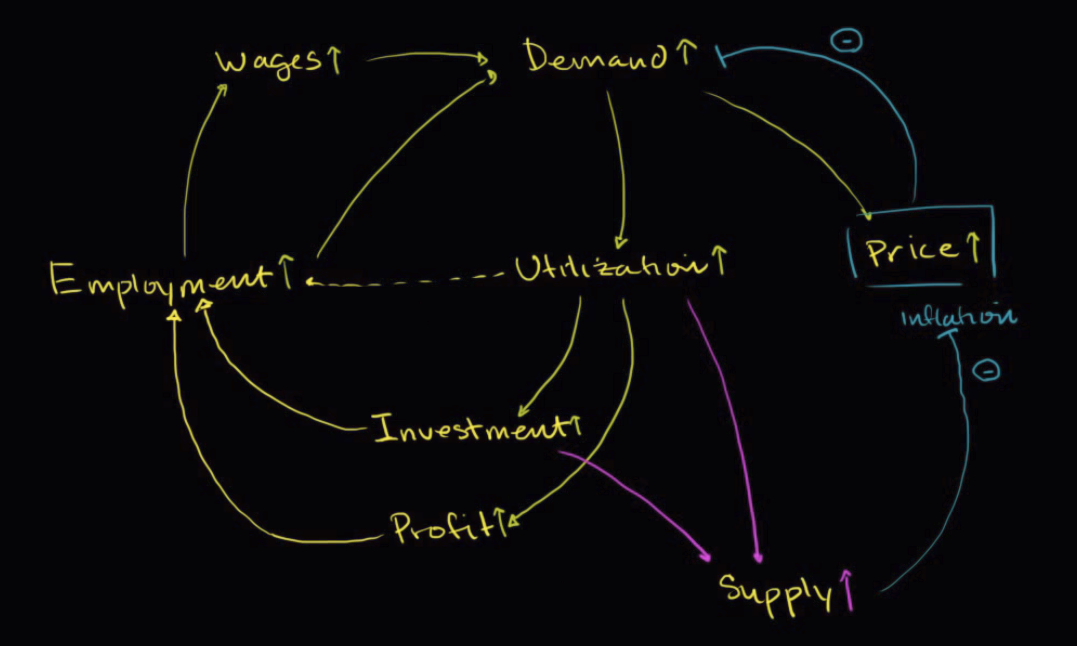
\includegraphics[width=0.8\textwidth]{images/good_economy.png}
\caption{A good economy}
\label{fig:good_economy}
\end{figure}

Another scenario is when the supply of a certain product suddenly decreases. Here, prices would go up, but there is not an increment in the demand because there is no increment on wages and not more profit. The result is stagflation, where prices are high, but people do not tend to spend more.

Hyperinflation happens when a central bank starts printing money because the government has no other way of getting money. This leads to higher prices as more money is available. This in turn leads to printing more money as the employees would start demanding more money to pay the products. If the price of a product keeps going up, then it's better to buy it and keep it (hoarding) as it will value more in the future. If no one wants to sell a product but everybody wants to buy it as it is getting value, there will be higher and higher demand increasing prices even more. Famous examples are: Weimar Germany after WWI, Zimbabwe, Hungary after WWII.

\section{Real and nominal return}

Assume one year ago I put a sum of money $S$ into the bank with an interest rate $r$, which means I have today $S' = S\cdot (1+r)$. I can think of $d = S'-S$ as my profit of this annual investment. But is it really true? In one year we may have a different inflation, suppose it has increased of $i$. This means that a product priced $S$ one year ago, is now $S_i = S \cdot i$. Hence, the return in today's money is $d_i = S' - S_i$ and the real return is:

\begin{equation}\label{eq:real_return}
r_i = \dfrac{d_i}{S_i} = \dfrac{S' - S_i}{S_i} = \dfrac{(1+r)}{(1+i)}-1.
\end{equation}

Equation \ref{eq:real_return} can also be seen as: the nominal interest rate $(1+r)$ is equal to the real interest rate $(1+r_i)$ compounded by the inflation rate $(1+i):$

\begin{equation}\label{eq:nominal_rate}
r+1 = (r_i + 1)(1+i).
\end{equation}


\section{Capacity utilization and inflation}

When starting up a business we have an initial capital $S$ and then we start thinking about the operating costs per year $C_{op}$, the costs for producing the good $C_g$, the price $p$ of the good, the number of goods you estimate to be able to produce per year $N_y$. After one year you, sold $N$ goods with a revenue $R = N \cdot p$. Considering the costs of goods $COGS = C_g \cdot N$, your gross profit $P_g = R - COGS$. Deducting the operating costs, also called overhead, you get the operating profit $P_{op} = P_g - C_{op}$. 
In an open market with competition, if a business is using a small part of its capacity, it should lower the prices so that it'll use more of its capacity. If it is instead using a big part of its capacity, it should increase the prices and maybe make more profits. In general, utilization of capacity determines inflation or deflation. Usually, capacity is correlated to demand and velocity (see below). When the average utilization is around 80-85\%, it means there is someone at 70\% and someone at 95\%. The latter ones usually start increasing prices entering a phase with increasing inflation. This can be seen in Figure~\ref{fig:inflation_utilization}. Dotted-light-blue lines represent 80-85\% of utilization. The light-blue bottom line is zero inflation. Below that line we have deflation. This means that from the '70s we've always had inflation. Interesting to notice that right before the '90s there was high utilization, but it didn't exceed 85\% and inflation didn't explode.

\begin{figure}[h!]
\centering
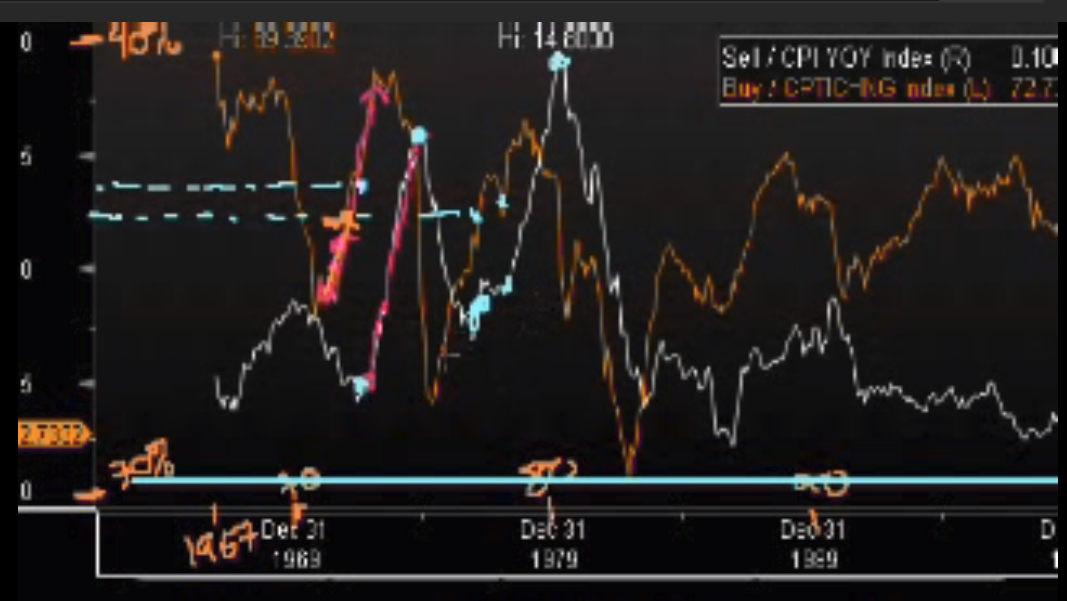
\includegraphics[width=0.8\textwidth]{images/inflation_utilization.png}
\caption{Inflation (white) and utilization (orange). Dotted-light-blue lines represent 80-85\% of utilization. The light-blue bottom line is zero inflation. High utilization is followed by high inflation twice between 1969 and 1979.}
\label{fig:inflation_utilization}
\end{figure}

On the other hand, an increase in money supply from central banks does not necessarily lead to higher demand―hence higher utilization―in that the consumer might fear to spend and thinks the market is not favourable somehow.
An equation used to describe this situation is the following:

\begin{equation}\label{eq:money_supply}
M \cdot v = p \cdot Q
\end{equation}

where $M$ is the total money supply, $v$ is the velocity of money i.e., how often it is exchanged on the market, $p$ is the average price of goods and $Q$ is the total quantity of goods and services. One can see that higher money supply lead to higher prices or higher utilization only if velocity is constant, but that's not always the case.


\begin{figure}[h!]
\centering
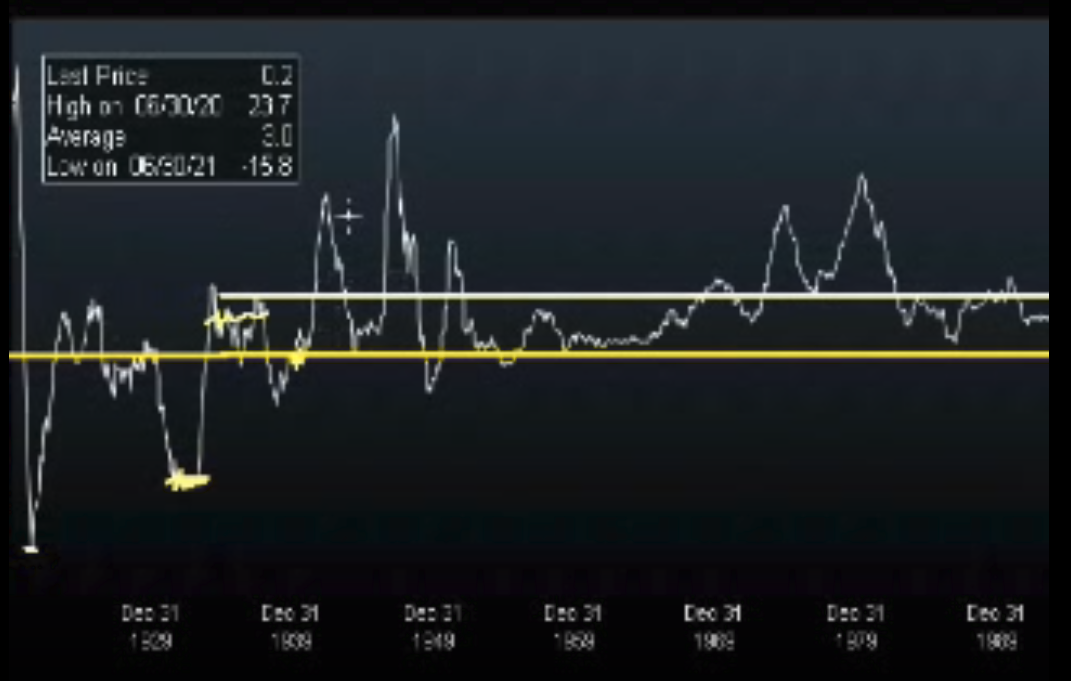
\includegraphics[width=0.8\textwidth]{images/deflation_inflation.png}
\caption{Inflation. Yellow line is zero inflation, white line is 5\% inflation, usually considered critical threshold. Few deflationary periods happened in the last century. Among them, the Great Depression in the '30s.}
\label{fig:deflation_inflation}
\end{figure}

Let's assume a country has an annual output, or Gross Domestic Product of $GDP$, a percentage of it is consumed\footnote{Consumption is spending money on stuff that will lose value, for example, when you buy a sofa the value of the sofa goes down so the money effectively disappears and you can't get it back. The opposite of consumption is investment, where you spend money on something that will (hopefully) increase in value later on, so you get more money back.}, say $c$, and the rest is for savings. These savings are usually turned into investments for the next year so that the output can increase, meaning that people get paid more and spend more and the standard of living will go up. Generally, if there are no savings, there are no money for investment and the output will decrease. In 2007, the United States consumed more than their output meaning that they "borrowed" output from other countries, such as China. A realistic scenario is that the US bought products from China using USD as a currency and, as time goes by, the amount of dollars in China increases. But US dollars are not accepted in China, hence the Chinese end up with a lot of dollars to spend. What do they buy? They buy US bonds, essentially US debt. In addition, the US was not able to save as everything was consumed and if they need money for investments, again they have to borrow more output from other countries. High consumption, by itself, attracts foreign investments. The problem appeared when people were not able to pay their (home equity) loans. Banks lost money. Liquidity was gone. People could not borrow money, nor buy. Demand and consumption went down. Utilization went down. Prices went down. Wages went down. Deflationary cycle's fear was real. By printing money, the government tries to borrow money so that people start spending, demand and consumption go up again and inflation is back. 

If the output of a country is $GDP$, a fraction of it is for taxes, another fraction is for businesses' savings and the rest is disposable income. In Figure \ref{fig:saving_rate}, the saving rate is represented from 1972 to 2008 and one can clearly see the decreasing trend. Before this period, the saving rate was around 10\%. One theory is that in the last years people had perceived savings near 10\%, but real saving was dropping because people were using credit to make more purchases than they should have been. As we approached zero, it all started collapsing because people finally realized that the credit they used to buy stuff was actually backed from savings that didn't really exist. After that, people was unable to spend and average savings went up again as depicted in the last part of the plot because people were not able to spend more than what they had (previously they were offsetting the savers).

\begin{figure}[h!]
\centering
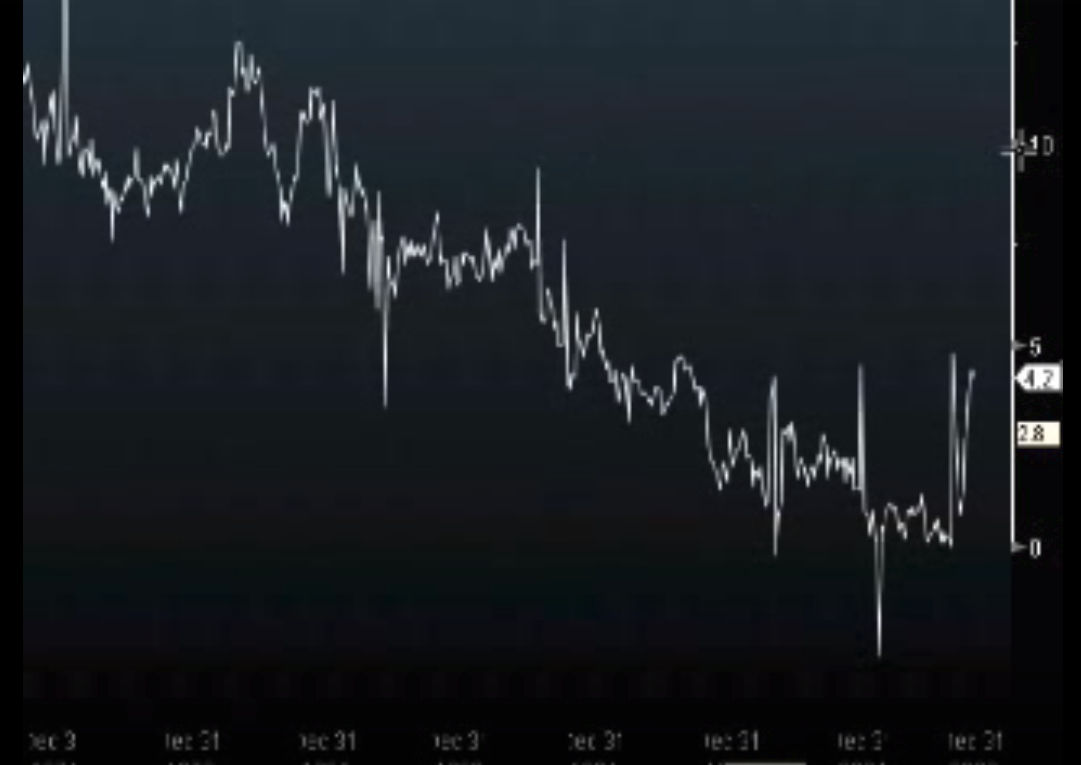
\includegraphics[width=0.8\textwidth]{images/savings.png}
\caption{Saving rate from 1972 to 2008.}
\label{fig:saving_rate}
\end{figure}
